\chapter{Implementation}

The implementation section below will explain what technologies were used and how they were implemented into ChatX.

\section{Server}

The Server is written in C\#, it is the part of the system that handles the users and which rooms they are in. The server is split up with the three layer architecture. Model, Controller and GUI. 

%The Model layer consists of four classes, User, Room, Message and Lobby. User class is used to handle the users in the system. The Room class keeps track of which users are in which rooms and allows them to send messages between them in the rooms. The Message class is what users use to send chat messages with. The lobby class works almost the same as the room class, it's a room class that will never be deleted and where all users are put in when they log in.%

The Model layer consists of two classes, User and Room. The User class is used to handle the users in ChatX. The Room class keeps track of which Users are in it.


The server has an interface which contains the necessary methods to implement any messaging queue system if RabbitMQ should ever be replaced. For now, RabbitMQ is the message queue system that listens to commands from the service and, depending on what the service requests from the server, sends messages back to the service.

The Controller is where the servers logic has been implemented. It has one class: ServerController. It keeps track of how many users are online in the system, which rooms those users are in, how many rooms there are and also which usernames are already taken. ServerController uses the singleton pattern, meaning there can only be one instance of ServiceController on the server. This has been done because otherwise it would be difficult to handle which users and rooms belong to which instances. Service Controller has a event handler that checks what commands it recieves from Service, the event handler looks into what command the message has and sends it to the appropriate method. ServerController consists of seven methods, JoinRoom, SendMessage, RequestRooms, LoginRequest, VerifyAndLockUsername, and ReleaseUsername. Whenever a user logs in, a socket connection is created between the Server and users logging in their rooms, which allows users to communicate with eachother. Lastly ServerController makes use of the same Config file used in the Service. It helps showing how the messages from RabbitMQ should be understood for both sides.



The GUI for the server is to control the server. It can turn on the Server, so it starts listening for any incoming messages from the Service, and it can be turned off. It can also connect to a specified service IP.


\section{Webservice}
The webservice is written in C\#, and is implemented using Windows Communication Foundation (WCF). 

The function of webservice is to be a broker between the client and the server(s); whenever a client interacts with the system, be it sending a message or requesting a list of rooms, it needs to go through this service. The service will then  contact the server(s) through a queue system, currently RabbitMQ, through which the servers also sends their response. The communication can be seen in figure \ref{fig:Communicationdiagram}.

The service consists of:
\begin{itemize}
 \item The exposed functionality available to the clients. This is done through the usual way with an interface as the service contract, and an implementation.

 \item A server distributor. The idea of this is to handle what servers are available, what their IP's are and what port-numbers the socket-connections should be created to go to. 
 
 \item A message queue driver. This handles all functionality related to the messaging queue system.
 
 \item A config class file. This file statically contains the formats of the actual messages send and received through the messaging queue system.

\end{itemize}

The first three of the above items all inherit from the interfaces IChatXService, IServerDistributor and IMQDriver respectively. The first interface is implemented, as this is common, good practice for services. The next two has interfaces to make it easier to replace the actual implementations at a later state of development and even deployment. At the moment, the implementation of the server distributor only distributes to one server, and the only messaging system implementation uses RabbitMQ. But since the implementations are coded against an interface, the only change needed to switch to another implementation is at the initialization of the object.
Below, in figure \ref{fig:ServiceArchitecture}, the service is illustrated:

\begin{figure}[h]
	\centering
	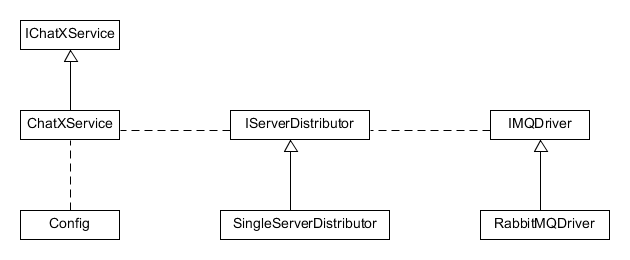
\includegraphics[width=0.7\linewidth]{img/ServiceArchitecture}
	\caption[Communication-diagram]{ChatX Service Architecture}
	\label{fig:ServiceArchitecture}
\end{figure}

The lines between ChatXService, IServerDistributor and IMQDriver are dotted to illustrate the statelessness of the service.

%\section{RabbitMQ}
%